\chapter{Анализ предметной области}

%%%%%%%%%%%%%%%%%%%%%%%%%%%%%%%%%%%%%%%%%%%%%%
\section{Классификация САРР}
Системы автоматического распознавания речи (САРР, англ. ASR -- Auto matic Speech Recognition) помогают машинам интерпретировать устную речь и автоматизировать задачи человека, например поиск в интернете, набор текста и тд. Одним из наиболее сложных моментов в разработке таких систем является довольно широкая междисциплинарность задачи, то есть затрагиваются вопросы теории обработки сигналов, математического анализа, психологии, теории коммуникаций, а также лингвистики.

Системы автоматического распознавания речи можно классифицировать по основным аспектам \cite{classif}.К таким аспектам можно отнести следующие. 
\begin{enumerate}
	\item Тип речи.
	\begin{enumerate}
		\item Спонтанная речь.
		
		Спонтанную речь можно рассматривать как речь, которая звучит естественно (с эмоциями, с внезапными паузами).
		
		\item Непрерывная речь. 
		
		Непрерывная речь -- это обычная человеческая речь без пауз между словами. Этот вид значительно затрудняет машинное понимание речи.
		
		\item Связные слова.
		
		Такие слова требуют минимальные паузы между высказываниями. Речь должна течь плавно.
		
		\item Изолированная речь.
		
		Такие системы направлены на распознавания конкретных голосовых команд, получаемых от пользователя.
		
	\end{enumerate}
	
	\item Размер словаря.
	\begin{enumerate}
		\item Маленькие словари.
		
		САРР с маленькими словарями (чаще до 500-1000 слов) необходимы для распознавания команд, получаемых от пользователя.
		
		\item Большие словари.
		
		Такие словари чаще всего используются в САРР слитной речи. Размеры достигают до десятков тысяч слов \cite{babin}.
	\end{enumerate}
	
	\item Персонализация.
	\begin{enumerate}
		\item Дикторозависимые.
		
		К классу систем, зависящих от диктора относятся системы, которые требуют предварительного обучения и в его процессе настраиваются на определенного диктора. При смене диктора в таких системах возникает необходимость полной перенастройки. 
		
		\item Дикторонезависимые.
		
		К классу систем, независимых от диктора относятся системы, которые 	работают вне зависимости от того, кто выступает в качестве диктора. Данные системы имеют возможность распознания речи любого диктора и не нуждаются в предварительном обучении.
		
	\end{enumerate}
	\item Структурные единицы. 
	
	В качестве структурных единиц могут выступать фразы, слова, фонемы. Системы, которые распознают речь, используя целые слова или фразы, называются системами распознавания речи по шаблону. Создание таких систем менее трудоемко, чем системы основанные на базе выделения лексических элементов (в таких системах структурными единицами являются фонемы). 
	
	\item Принцип выделения структурных единиц.
	
	В современных САРР используются несколько подходов для выделения структурных единиц из потока речи. 
	\begin{enumerate}
		\item Фурье-анализ. 
		
		Данный анализ предполагает разложение исходной периодической функции в ряд, в результате чего исходная функция может быть представлена как суперпозиция синусоидальных волн различной частоты \cite{fur_veivlet}.
		\item Вейвлет-анализ (от англ. wavelet -- <<маленькая волна>>). 
		
		Данный анализ раскладывает исходный сигнал в базис функций, которые характеризуют как частоту, так и время \cite{fur_veivlet}.
		\item Кепстральный анализ. 
		
		Данный анализ основан на выделении кепстральных коэффициентов на мел\footnote{Мел -- единица высоты звука \cite{kepstr}.}-шкале, называемых мел-частотными кепстральными коэффециентами. Кепстр -- это дискретно-косинусное преобразование амплитудного спектра сигнала в логарифмическом масштабе. 
	\end{enumerate}
	
	\item Механизм распознавания
	\begin{enumerate}
		\item Скрытые Марковские модели (СММ).
		
		СММ -- это модель, состоящая из $N$ состояний, в каждом система может принимать одно из $M$ значений какого-либо параметра. Матрицей $A = [a_{ij}]$ задаются вероятности переходов между состояниями из $i$ состояния в $j$ состояние. Вектором $B = [{b_j (k)}]$ задается вероятность выпадения какого-либо из $M$ значений параметра в каждом из $N$ состояний (выпадения $k$ значения параметра в $j$ состоянии). Вероятность того, что в начальные момент система окажется в $i$ состоянии определяется вектором $\pi = {\pi_i}$. Таким образом, СММ называется тройка $\lambda = ({A, B, \pi})$.  
		
		Модель называется <<скрытой>>, потому что последовательность, в которой пребывала система неважна. Другими словами такая система выступает в роли <<черного ящика>>, на вход которого поступает последовательность параметров, а на выход ожидаем модель, которая с максимальной вероятностью генерирует такую последовательность.
		
		\item Динамическое искажение времени.
		
		Алгоритм динамического искажения времени (Dynamic Time \newline Warping – DTW) является методикой эластичного сравнения вектора наблюдений с хранящимся шаблоном. По-другому можно сказать, что это мера подобия временных рядов, которая минимизирует эффекты временного сдвига, различного течения времени, а также обеспечивает непрерывное преобразование временных рядов для того, чтобы обнаружить одинаковые формы с различными фазами.
		
		\item Нейронные сети.
		
		С помощью нейронных сетей можно создавать самообучаемые и обучаемые системы распознавания речи. Некоторые факторы, которым должны отвечать такие системы: возможность контроля своих действий с последующей коррекцией, разработка системы заключается только в построении архитектуры системы.
		
	\end{enumerate}
	
	\item Назначение
	\begin{enumerate}
		\item Командные системы.
		
		Такие системы используют распознавания по шаблону (фразе или слову).
		
		\item Системы диктовки.
		
		Такие системы требуют более точного распознавания, то есть выделение лексических элементов. Также при интерпретации произнесенной фразы система полагается не только на то, что произносилось в данный момент, но и на фразы, сказанные ранее.
		
	\end{enumerate}
\end{enumerate}

Обобщив все выше перечисленное можно представить классификацию систем распознавания речи на рисунке \ref{fig:xray3}.

\begin{figure}[h!]
	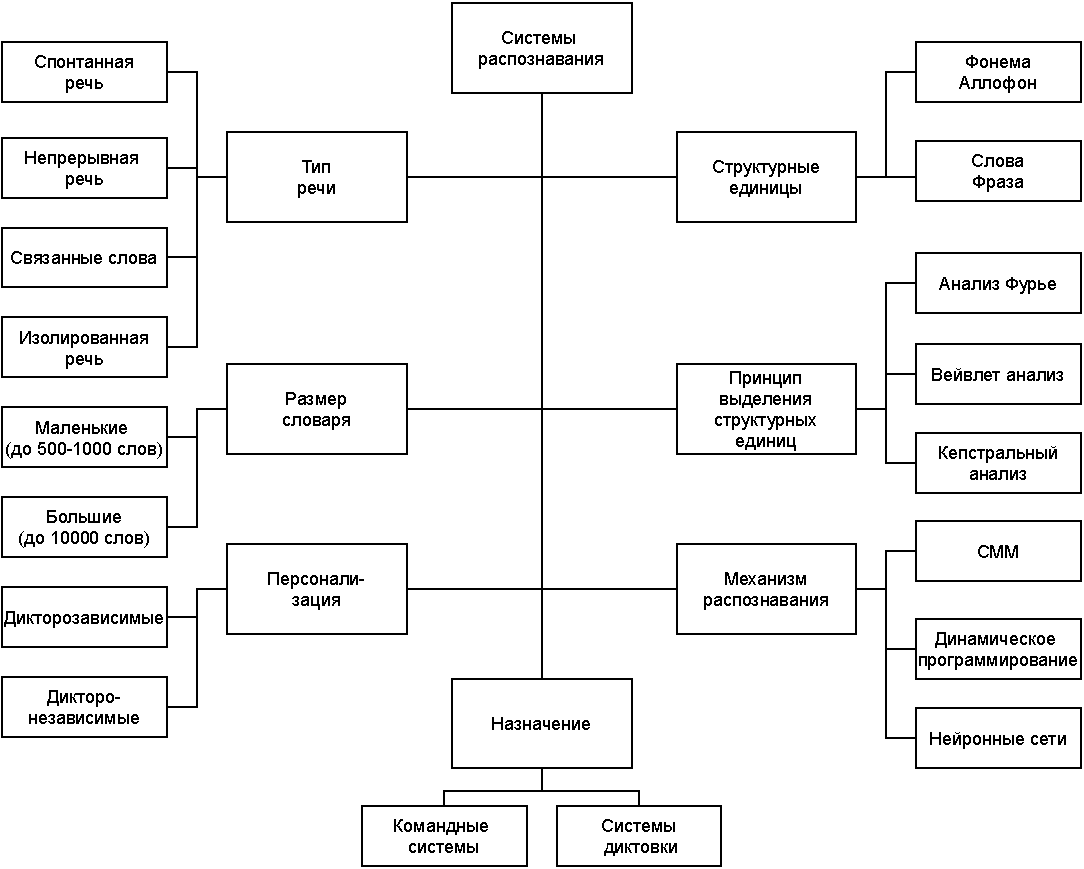
\includegraphics[pages=-, scale=0.9]{./inc/img/2.pdf}
	\caption{Классификация систем распознавания речи}  
	\label{fig:xray3}
\end{figure}
\newpage

%%%%%%%%%%%%%%%%%%%%%%%%%%%%%%%%%%%%%%%%%%%%%%
\section{Сложности в работе САРР}
Распознавание речи -- это задача, усложненная тем, что речь человека характеризуется высокой степенью изменчивости \cite{spr}. 

Причины этого следующие:
\begin{itemize}
	\item для одного и того же диктора произношения одних и тех же звуков (слов, фраз) будут отличаться длительностью произношения, интонацией. Часто это связано с изменением физического или эмоционального состояния человека, его настроения или условий, в которых он находится;
	\item произношение фонем сильно зависит от контекста, например наличие или отсутствие четкой артикуляции при разговоре;
	\item различные помехи (отражения звука, искажение микрофона, фоновый шум).
\end{itemize}

Отличием распознавания слитной речи от, например, отдельных команд или подготовленной речи, являются различные сбои в произношении \cite{rechsb2} \cite{rechsb1}. Очень сложно говорить гладко (не сбиваясь) и красиво оформлять свои мысли (четко и ровно составлять предложения), поэтому можно сказать, что основная особенность слитной речи -- это сбивчивость, наличие повторений, пауз, слов в упрощенной форме (разговорный стиль) \cite{slitrech}. 

Такие особенности зачастую являются препятствием для обработки речи техническими средствами, так как уловить особенности разговорной речи человека довольно сложно машине, поэтому необходимо либо разработать метод, на основе которого машина научиться распознавать речь человека, либо составлять сверхбольшой словарь слов или звуков, что довольно затратно по памяти \cite{slitrech}.

%%%%%%%%%%%%%%%%%%%%%%%%%%%%%%%%%%%%%%%%%%%%%%
\section{Нарушения и дефекты речи}
У людей с дефектами речи помимо выше описанных особенностей есть и другие, не менее важные, поэтому специальные системы распознавания речи должны также распознавать разные виды нарушения устной речи.

%Существует несколько классификаций нарушений:
%\begin{itemize}
%	\item клинико-педагогическая классификация.
%	\item психолого–педагогическая классификация.
%\end{itemize}

%В данной работе будут рассмотрены нарушения клинико-педагогической классификации \cite{narush}. 

Виды нарушения устной речи \cite{narush}.
\begin{enumerate}
	\item Нарушения внешнего оформления устной речи.
	\begin{enumerate}
		\item Дисфония -- отсутствие голоса или расстройство речи вследствие патологических изменений голосового аппарата: происходят различные изменения и нарушения в силе и тембре, выражающееся в охриплости, слабости голоса.
		\item Брадилалия -- медленный темп речи вследствие поражения головного мозга. Речь сильно замедляется, становится нечеткой, растягиваются гласные.
		\item Тахилалия -- быстрый темп речи, часто сопровождающийся повторением или пропуском слов, незамеченным говорящим. 
		\item Заикание -- нарушение речи, которое характеризуется частым повторением или пролонгацией звуков, слогов, слов, частыми остановками или нерешительностью в речи, разрывающее ее ритмическое течение.
		\item Дислалия -- нарушение звукопроизношения при нормальном слухе и нормальной иннервации речевого аппарата, которое проявляется в заменах, искажениях и смешениях звуков родной речи.
		\item Ринолалия -- нарушение произносительной стороны речи или тембра голоса, обусловленное анатомо-физиологическим поражением речевого аппарата: струя воздуха проходит не в ротовую, а в носовую полость, в которой происходит резонанс.
		\item Дизартрия -- нарушение произносительной стороны речи вследствие поражения центральной нервной системы. 
	\end{enumerate}
	\item Нарушения структурно-семантического оформления.
	\begin{enumerate}
		\item Алалия -- полное отсутствие или недоразвитие речи у детей при нормальном слухе и первично сохранном интеллекте.
		\item Афазия -- речевое расстройство уже сформировавшейся речи. Причинами могут быть перенесенные черепно-мозговые травмы, инфекционные заболевания нервной системой.
	\end{enumerate}
\end{enumerate}

Также стоит отметить, что нарушения речи могут встречаться в комплексе, например: заикание и дизартрия.

Выше перечисленные нарушения также являются препятствием для обработки речи техническими средствами. В разделе \ref{5000} будет приведен эксперимент из статьи \cite{primer}, в котором показано, что машина иногда не понимает, что говорит человек с нарушениями речи.


\section{Рассмотрение эксперимента} \label{5000}
В статье \cite{primer} проводится эксперимент работы трех платформ САРР \newline(Amazon, Google, IBM) для групп людей: с нейродегенеративными (медленно прогрессирующие, наследственные или приобретенные заболевания нервной системы, ведущими к различным симптомам -- к деменции \footnote{Деменция — это синдром, возникающий при поражении головного мозга и характеризующийся нарушениями в когнитивной сфере (восприятие, внимание, узнавание, память, интеллект, речь).}, нарушению движения, а в следствие чего к нарушениям речи) заболеваниями и здоровых.

Записи чтения текста были расшифрованы с помощью САРР и вручную, затем сравнены. Точность расшифровки измерялась как доля верно распознанных слов. 

Результат эксперимента ожидаем: точность расшифровки САРР для здоровых людей выше, чем для людей с заболеваниями (рассматривались 3 группы людей, с различными заболеваниями: с рассеянным склерозом и с атаксией Фридрейха \footnote{Атаксия Фридрейха — генетическое заболевание, связанное с нарушением транспорта железа из митохондрий и протекающее с преимущественным поражением клеток центральной и периферической нервной системы.}). При этом при увеличении продолжительности болезни, точность расшифровки САРР снижалась. 

Часть результата приведена на рисунке \ref{fig:xray1}

Обозначения: 
\begin{itemize}
	\item Группа 1 -- группа здоровых людей;
	\item Группа 2 -- группа людей с рассеянным склерозом;
	\item Группа 3 -- группа людей с заболеванием ''Атаксия Фридрайха''.
\end{itemize}
\begin{figure}[h]
	\begin{center}
	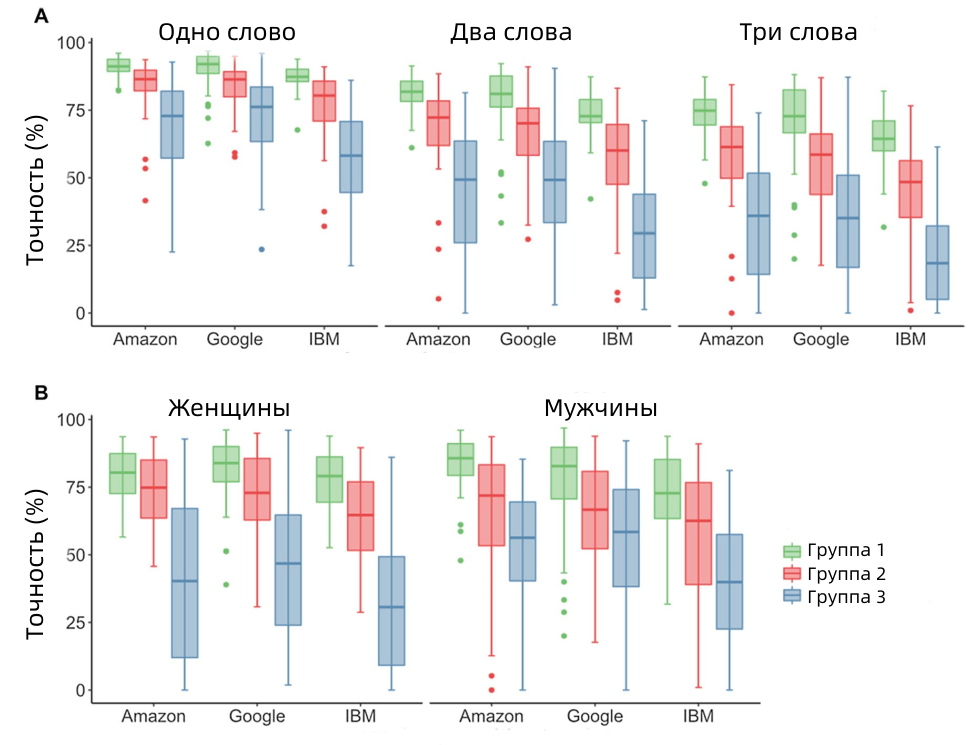
\includegraphics[pages=-, scale=0.45]{./inc/img/primer2.png}
	\caption{Результаты эксперимента из статьи \cite{primer}}  
	\label{fig:xray1}
\end{center}
\end{figure}
\newpage


Как видно из эксперимента, системы распознавания речи работают с ошибками для людей с нейро-дегенеративными заболеваниями.


%%%%%%%%%%%%%%%%%%%%%%%%%%%%%%%%%%%%%%%%%%%%%%
\chapter{Классификация существующих методов}
\section{Основные характеристики речевых сигналов}
Все особенности речевых сигналов можно условно разделить на то, что схоже у определенного состава людей, например, отношение к какой-либо языковой группе, и на то, что индивидуально для каждого человека -- особенности, выраженные в физической индивидуальности речи, произношении, тембре голоса. \cite{chastot} \cite{chastot2}

Для того, чтобы сформировать перечень спектральных\footnote{Спектр сигнала — это совокупность простых составляющих сигнала с определенными амплитудами, частотами и начальными фазами.\cite{spektr}} характеристик в расчет берется только первая гармоника\footnote{Гармоники — это высокочастотные сигналы, накладываемые на основную частоту, то есть частоту цепи, и которые достаточны для искажения формы волны.\cite{spektr}}. 

В соответствии с измеряемой величиной основные спектральные характеристики разделены на следующие группы. \cite{chastot} \cite{chastot2} \cite{signal}
\begin{enumerate}
	\item Частотные характеристики.
	\begin{enumerate}
		\item Частота основного тона -- частота первой гармоники спектра (Гц\footnote{Герц (Гц, Hz) -- единица частоты периодических процессов.}).
		\item Период основного тона (мс).
		\item Количество побочных гармоник (Гц).
		\item Нижняя и верхняя частота спектра (Гц).
		\item Частотный диапазон (Гц).
		\item Частота максимального уровня спектральной плотности (Гц).
	\end{enumerate}
	\item Энергетические характеристики.
	\begin{enumerate}
		\item Нижний уровень громкости речи (дБ\footnote{Децибел (дб) --  относительная единица измерения, соответствующая одной десятой бел (В).}).
		\item Верхний уровень громкости речи (дБ).
		\item Динамический диапазон (дБ).
		\item Амплитуда основного тона (дБ).
	\end{enumerate}
	\item Временные характеристики.
	\begin{enumerate}
		\item Длительность звука речи (мс).
		\item Длительность пауз речи между словами/фразами (мс).
		\item Скорость звуков речи (звуков/с).
		\item Темп речи (слов/мин).
		\item Плотность речи -- отношение времени наличия звука к
		полному времени речевого сигнала (\%).
	\end{enumerate}
\end{enumerate}

%%%%%%%%%%%%%%%%%%%%%%%%%%%%%%%%%%%%%%%%%%%%%%
\section{Методы извлечения речевых характеристик}
В системах распознавания речи одну из главных ролей играет извлечение признаков (частотной характеристики), при этом характеристики сигналов возбуждения чаще всего отбрасываются. 

Извлечение признаков -- это процесс удаления ненужной и избыточной информации и сохранение только полезной информации. Цель такого действия состоит в том, чтобы определить набор свойств (параметры), путем обработки формы сигнала поступившего на вход системе.  Извлечение признаков включает процесс преобразования речевых сигналов в цифровую форму и измерение важных характеристик сигнала, например, энергии или частоты, и дополнение этих измерений значимыми производными измерениями. \cite{isvparam1} \cite{isvparam2}.

Методы извлечения признаков удобно применять при обработке речи с неправильным произношением звуков, так как их можно адаптировать, извлекая нужные параметры, которые потребуются в дальнейшем.

\subsection{Линейно-предсказывающее кодирование}
Линейно-предсказывающее кодирование (англ. Linear prediction coding \newpage(LPC)).

%Линейное предсказание уже продолжительное время остается одним из основных подходов к задачам цифровой обработки речи. 

Принцип метода линейного предсказания состоит в том, что участок речевого сигнала можно аппроксимировать линейной комбинацией предыдущих участков сигнала. Предполагается, что речь создается возбуждением линейного изменяющегося во времени фильтра (речевого тракта) случайным шумом для невокализованных речевых сегментов или последовательностью импульсов для голосовой речи \cite{methodisb}.

Процесс речеобразования описывается линейной системой с переменными параметрами и передаточной функцией\footnote{Передаточной функцией называется отношение изображения выходного воздействия к изображению входного при нулевых начальных условиях. \cite{peredfunc}} \eqref{H}.
\begin{equation}
\label{H}
H(z) = \frac{G}{1 - \sum_{k = 1}^{p} a_k z^{-k}},
\end{equation}
где $G$ -- коэффициент усиления, $a_k$ -- коэффициент предсказания, $p$ -- порядок линейного предсказания.

Зависимость $n$-го отсчета речевого сигнала $s(n)$ от сигнала возбуждения $u(n)$ выражается в виде \eqref{s}
\begin{equation}
\label{s}
s(n) = \sum_{k = 1}^{p} a_k s(n - k) + G u(n)
\end{equation}

Линейный предсказатель с коэффициентами $a_k$ представляется в виде системы с сигналом на выходе, который рассчитывается по формуле \eqref{s1}
\begin{equation}
	\label{s1}
	s(n) = \sum_{k = 1}^{p} a_k s(n - k)
\end{equation}

Суть данного метода заключается в нахождении \textit{линейных коэффициентов предсказания} по речевому сигналу с минимизацией погрешности, которую можно определить по формуле \eqref{s3}
\begin{equation}
	\label{s3}
	e(n) = s(n) - \sum_{k = 1}^{p} a_k s(n - k)
\end{equation}

Недостатком этого метода является то, что он сильно зависит от точности произношения. Поэтому, можно сказать, что данный метод не подходит для решения задачи распознавания речи у людей с дефектами речи.

\subsection{Мел-частотные кепстральные коэффициенты} \label{1}
Мел\footnote{Мел -- единица высоты звука. \cite{kepstr}}-частотные кепстральные\footnote{Кепстр (cepstrum) — это результат дискретного косинусного преобразования от логарифма амплитудного спектра сигнала. \cite{kepstr}} коэффициенты (англ. Mel frequency \newline Cepstral Coefficient (MFCC)).

Мел-частотный анализ представляет частоты речи с позиции психоакустического \footnote{Психоакустика - это наука, изучающая психологические и физиологические особенности восприятия звука человеком. \cite{psih}} параметра слуха – высоты тона. Высота тона определяет, насколько высоким или низким кажется тон слушателю. Связь между частотой звука и его высотой представлена на рисунке \ref{fig:xray}. \cite{methodisb} \cite{methodisb2}

Перевод частоты из Герц в Мел осуществляется по формуле  \eqref{s1}
\begin{equation}
	\label{s1}
	Mel(f) = 2595 * \log_{10}{1 + \frac{f}{700}},
\end{equation}
где $f$ -- частота в Герцах, $Mel$ -- частота в мелах.

\begin{figure}[h!]
	\begin{center}
	
\includegraphics[pages=-]{./inc/img/1.pdf}
	\caption{Связь между частотой звука и его высотой}  
	\label{fig:xray}
\end{center}
\end{figure}

Построение признаков MFCC начинается с процедуры разбиения входного сигнала на временные окна небольшой длины.
	
Пусть $N_{FB}$ -- количество фильтров (обычно используют порядка 24 фильтров), ($f_{low}$, $f_{high}$) -- исследуемый диапазон частот. Тогда данный диапазон переводят в шкалу мел, разбивают на $N_{FB}$ равномерно распределенных частей и вычисляют соответствующие границы в области линейных частот.

Следующие преобразования применяются к каждому кадру. 
\begin{enumerate}
	\item Предварительная фильтрация.
	
	Суть данного шага -- уменьшение негативных эффектов, которые возникают во время обработки звукового сигнала. 
	
	\item Применение весовой оконной функции.
	
	Такая функция применяется с целью уменьшения краевых эффектов, возникающих в результате разбиения сигнала на кадры.
	
	\item Подсчет логарифма энергии спектра для набора треугольных мел-\newline частотных фильтров.
	
	Также стоит отметить, что если использовать вместо мел-шкалы линейное преобразование, то результатом вычислений будут являться так называемые линейно-частотные кепстральные коэффициенты \ref{2}.
	
	\item В конце всех преобразований к коэффициентам применяется дискретное косинусное преобразование. В качестве итоговых значений берутся первые несколько коэффициентов дискретного косинусного преобразования.
	
\end{enumerate}

Положительные моменты при использовании кепстральных коэффициентов:
\begin{itemize}
	\item спектр проецируется на специальную Мел-шкалу, позволяя выделить наиболее значимые для восприятия человеком частоты;
	\item количество вычисляемых коэффициентов может быть ограничено любым значением.
\end{itemize}


	
\subsection{Кепстральные коэффициенты на основе линейного предсказания} \label{2}
Кепстральные коэффициенты на основе линейного предсказания (англ. Linear prediction cepstral coefficient (LPCC)). 

Метод LPCC похож на MFCC во многом, но главное отличие в том, что он использует линейную шкалу перевода частоты звука в его высоту, воспринимаемую мозгом. Этот способ хорошо работает в области низких частот, так как в этой зоне зависимость высоты звука от его частоты практически линейна. Данная особенность позволяет достичь схожих	результатов при извлечении признаков в области низких частот. \cite{methodisb}


Суть линейного предсказания заключается в том, что линейной комбинацией некоторого количества предшествующих отсчетов можно аппроксимировать текущий отсчет, то есть
\begin{equation}
	\label{H}
	x(n) = \sum_{k = 1}^{p} a_k x_{n-k},
\end{equation}
где $a_k$ -- коэффициент предсказания, $p$ -- порядок линейного предсказания.

На основе полученных коэффициентов линейного предсказания рассчитываются кепстральные коэффициенты по формуле \eqref{s5}. Причем таких коэффициентов может быть сгенерировано больше, чем самих коэффициентов линейного предсказания.
\begin{equation}
	\label{s5}
	c_n = \left\{\begin{matrix}
		a_n + \sum_{k=1}^{n-1} \frac{k}{n} c_k a_{n-k}& 1\leq n\leq p\\ 
		\sum_{k=n-p}^{n-1} \frac{k}{n} c_k a_{n-k}& n>p
	\end{matrix}\right.
\end{equation}

%Алгоритм можно разделить на несколько этапов:
%\begin{enumerate}
%	\item Речевой сигнал проходит предобработку фильтром, который усиливает высокие частоты спектра, которые в свою очередь уменьшаются в процессе воспроизведения речи.
%	\item Сигнал делится на одинаковые последовательные перекрывающиеся временные участки -- фреймы. С помощью преобразования Фурье для каждого участка находится среднее значение частот.
%	\item Производится математические вычисления, а именно берется логарифм от полученного ранее значения и выполняется дискретное косинусное преобразование.
%\end{enumerate}
	
Например, для сигнала может быть использовано около 12 коэффициентов линейного предсказания, из которых может быть получено порядка 18 кепстральных коэффициентов. \cite{methodisb2}



\subsection{Дискретное вейвлет-преобразование}
Дискретное вейвлет-преобразование (Discrete Wavelet Transform (DWT)).

Для наиболее информативного анализа сложных реальных сигналов необходима обработка как по частотным, так и по временным характеристикам, а также достоверное представление уровней детализации для обнаружения закономерностей. 

При обработке данных в современных пакетах математической обработки данных может выполняться дискретизированная\footnote{Дискретизация — в общем случае — представление непрерывной функции дискретной совокупностью ее значений при разных наборах аргументов. \cite{diskretiz}} версия непрерывного вейвлет-преобразования с заданием дискретных значений параметров $(a, b)$ вейвлетов\footnote{<<Вейвлет>> (wavelet) в переводе с английского означает <<маленькая (короткая) волна>>.} с произвольным шагом $\Delta a$ и $\Delta b$.

Результатом является избыточное количество коэффициентов, которое намного превосходит число коэффициентов, которые могут использоваться для выявления тонких особенностей исследуемых сигналов. 

Дискретное вейвлет-преобразование оперирует с дискретными значениями параметров $a$ и $b$, которые задаются, как правило, в виде степенных функций \eqref{f1}
\begin{equation}
	\label{f1}
	a = a_0 ^{(-m)}, b = k * a_0 ^{(-m)}
\end{equation}
где $m$ -- параметр масштаба, $k$ -- параметр сдвига.

Число использованных вейвлетов по масштабному коэффициенту $m$ задает уровень декомпозиции сигнала, при этом за нулевой уровень $(m = 0)$ обычно принимается сам сигнал.

%Идея применения вейвлетов состоит в многомасштабной обработке сигнала, т. е. в анализе сигнала в разном увеличении с разной степенью детализации.  \cite{methodisb2} \cite{signal2}

Недостатком вейвлет-преобразований можно считать их относительную сложность расчетов. 

Достоинством можно считать детальный разбор поступающего сигнала, что позволяет выявить множество тонких моментов. Именно поэтому данный метод подходит для решения задачи распознавания речи у людей с дефектами речи больше, чем методы, описанные в разделах \ref{1} и \ref{2}.

На рисунке \ref{fig:class} приведена классификация ранее рассмотренных методов извлечения частотных характеристик.

\begin{figure}[h]
	\begin{center}
	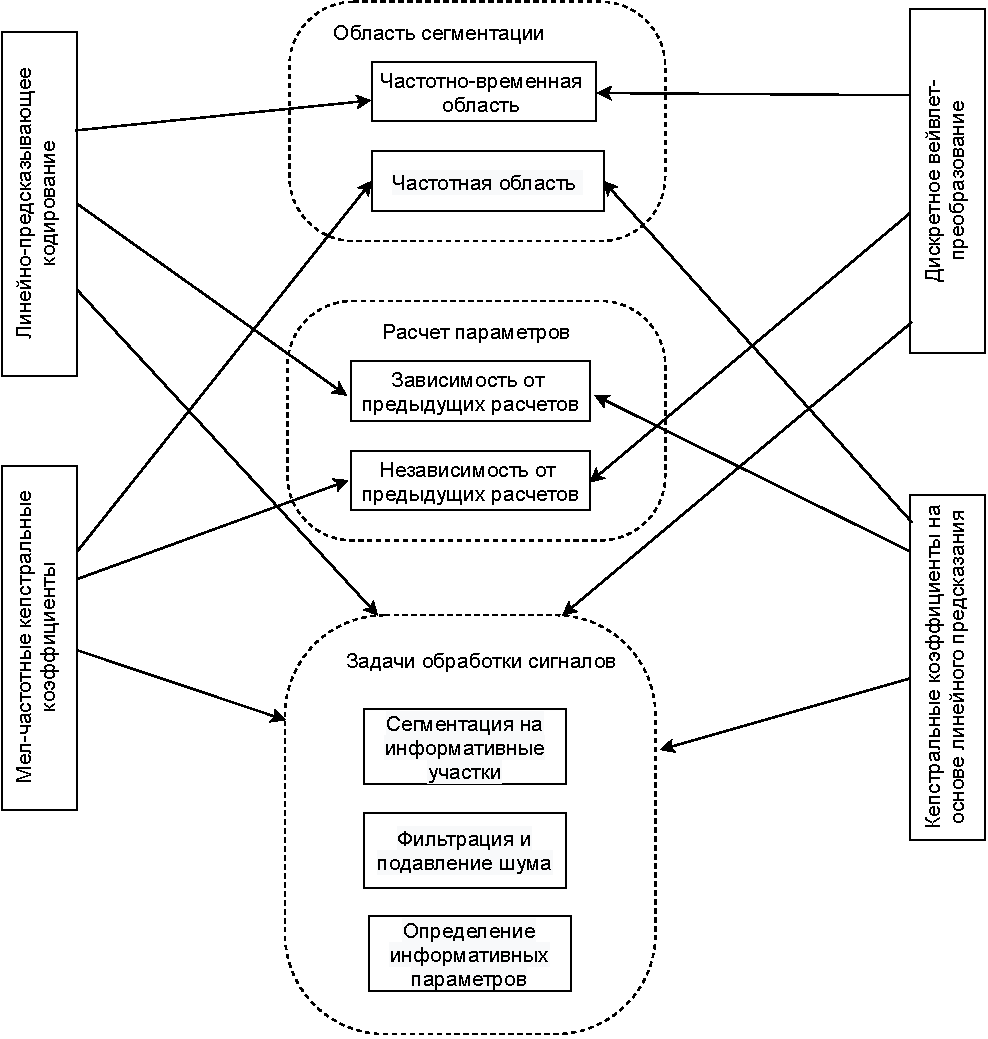
\includegraphics[pages=-, scale=0.85]{./inc/img/4.pdf}
	\caption{Классификация методов извлечения частотных характеристик}  
	\label{fig:class}
\end{center}
\end{figure}


